\chapter{Interacción de lípidos con los segmentos TM-IC de la integrina $\alpha$IIb$\beta$3 en bicapas lipídicas}\label{chap:dm}

El ambiente lipídico puede regular la función de proteínas de membrana a través de cambios macroscópicos y de largo alcance de sus propiedades, como fluidez, compresibilidad, radio de curvatura, o por interacciones específicas lípido-proteína. De la misma manera, las proteínas pueden modificar las propiedades del ambiente lipídico. Particularmente, las proteínas de transmembrana pueden inducir la formación de un ``anillo'' de lípidos a su alrededor. Los lípidos que se encuentran en este anillo disponen de menor libertad de movimiento comparado a los lípidos que se encuentran más alejados, también su orientación respecto a la normal de la bicapa se podría ver afectada según cuánto interaccione con la proteína \citep{Lee2011,Lee2003}.

\section{Simulaciones de dinámica molecular y el modelo grano grueso}

 Las simulaciones de \ac{dm} son una herramienta poderosa que permite explorar las interacciones proteína-proteína y lípido-proteína a nivel atómico. Cada vez son más las áreas de investigación que llevan a cabo estudios con la ayuda de las simulaciones atomísticas. Ésto ha sido posible con la ayuda de bases de datos de estructura de proteínas como PDB \citep{Berman2000}, junto a el incremento del tiempo de simulación como consecuencia de la mejora de hardware y nuevos modelos matemáticos que permiten describir apropiadamente un sistema de estudio. Sin embargo, las simulaciones de \ac{dm} a resolución atomística sigue siendo un desafío en términos de costo computacional y tiempo de simulación si el objetivo se trata de ver efectos como la conformación de una proteína, orientación en una membrana, conformación de los lípidos alrededor de la proteína, que solo son observables en el orden de los microsegundos. Es por esto que el uso del método de \acf{cg} es ampliamente utilizado en la biofísica computacional para la investigación de interacciones lípido-proteína. A diferencia de las simulaciones atomísticas, en \ac{cg} Martini se definen partículas que representan las propiedades de cuatro átomos pesados.
  
%%%%%%%%%%% Figura %%%%%%%%%%%%
\begin{figure}[t!]
    \centering
	\includegraphics[width=0.80\linewidth, height=0.4\textheight, keepaspectratio]{fig/02_dm/pept_AT_CG.png} 
	\caption[Conversión de átomo integrado a grano grueso del heterodímero $\alpha$IIb$\beta$3]{Conversión de átomo integrado a grano grueso del heterodímero $\alpha$IIb$\beta$3. A) Esquema general de la integrina  $\alpha$IIb$\beta$3 donde se identifica los dominos \ac{ec}, \ac{tm} e \ac{ic} (PDB: 1JV2 + 2KNC). B) Estructura secundaria a escala atomística de los segmentos \ac{tm}-\ac{ic} de la integrina (PDB: 2KNC). C) Mapeo de cada péptido de modelo atomístico a grano grueso Martini. Los colores de las partículas se corresponde con las propiedades fisicoquímicas, ver \textbf{figura} \ref{tab:tabla_aa}.}
      \index{aa_cg}
    \label{fig:aa_cg}
\end{figure}
%%%%%%%%%%%%%%%%%%%%%%% Fin %%%%%%%%%%%%%%%%%%%%%%%% 

 La \textbf{figura} \ref{fig:aa_cg}A muestra la estructura de la integrina $\alpha$IIb$\beta$3 (segmento extracelular, transmembrana y citoplasmático). En la \textbf{figura} \ref{fig:aa_cg}B-C la conversión de átomo integrado a grano grueso de los segmentos TM-IC. De forma similar la \textbf{figura} \ref{fig:aa_cg_lipid} muestra la conversión a grano grueso de una molécula de \ac{popc}. Para el mapeo en grano grueso de cada aminoácido se tuvo en cuenta la  \textbf{figura} \ref{tab:tabla_aa}.

%%%%%%%%%%% Figura %%%%%%%%%%%%
\begin{figure}[b!]
\vspace{0.5cm}
    \centering
	\includegraphics[width=0.60\linewidth, height=\textheight, keepaspectratio]{fig/02_dm/lipid_AT_CG.png} 
	\caption[Mapeo de átomo integrado a grano grueso de POPC]{Mapeo de átomo integrado a grano grueso de molécula de \ac{popc}.}
      \index{aa_cg_lipid}
    \label{fig:aa_cg_lipid}
\end{figure}
%%%%%%%%%%%%%%%%%%%%%%% Fin %%%%%%%%%%%%%%%%%%%%%%%%

Se generaron cuatro sistemas de bicapas lipídicas con 500 moléculas de lípido y un heterodímero \ac{tm}-\ac{ic} cada uno. En la \textbf{tabla} \ref{tab:cg_simulation} se observan los sistemas simulados \ac{dm} de los segmentos \ac{tm}-\ac{ic} de integrinas $\alpha$IIb$\beta$3 en bicapas lipídicas. Cada membrana consiste en 500 lípidos (250 por hemicapa), el heterodímero $\alpha$IIb$\beta$3, moléculas de agua (partículas poralizables, PW) y los contraiones NaCl 0.15 M para alcanzar la electroneutralidad del sistema. La membrana de \ac{dppc} se simuló a 360 K para llevar el sistema al estado líquido cristalino \citep{Leekumjorn2007} y de esa manera poder realizar comparaciones con los otros sistemas, además, darle movilidad a los lípidos y a los péptidos. 

La \textbf{figura} \ref{fig:cg_simulation}A-B muestra algunas capturas del sistema \ac{popc}-$\alpha$IIb$\beta$3 a tiempo cero (vista desde arriba y lateral). Las otras representaciones (\textbf{figura} \ref{fig:cg_simulation}C-D) muestran el seguimiento del heterodímero a diferentes tiempos durante la dinámica.

%%%%%%%%%%% Figura %%%%%%%%%%%%
\begin{figure}[H]
    \centering
	\includegraphics[width=0.9\linewidth, height=0.5\textheight, keepaspectratio]{fig/02_dm/esquema_cg_md.png} 
	\caption[Representación del sistema de bicapa lipídica con el heterodímero ensamblado]{Representación del sistema de bicapa lipídica con el heterodímero ensamblado. Membrana compuesta por lípidos de \ac{popc} donde las esferas \textcolor{gray}{grises} y \textcolor{mygreen}{verdes} representan las partículas de \textcolor{gray}{colina} y \textcolor{mygreen}{fosfato}, respectivamente; los bastones grises a las partículas de glicerol y cola hidrofóbica. El heterodímero \ac{tm}-\ac{ic} se muestra en \textcolor{red}{rojo ($\alpha$IIb)} y \textcolor{blue}{azul ($\beta$3)}. Los pequeños puntos dorados representan los iones (Na$^{\text{+}}$ y Cl$^{\text{--}}$), el agua se representa con la superficie azul clara.}
      \index{cg_simulation}
    \label{fig:cg_simulation}
\end{figure}
%%%%%%%%%%%%%%%%%%%%%%% Fin %%%%%%%%%%%%%%%%%%%%%%%%


\begin{table}[H]
\centering
\caption{Sistemas simulados en modelo CG Martini.}
\label{tab:cg_simulation}
\begin{tabular}{@{}lccclc@{}}
\toprule
\multicolumn{1}{l}{Sistema} &
  \begin{tabular}[c]{@{}c@{}}Temperatura\\  (K)\end{tabular} &
  \begin{tabular}[c]{@{}c@{}}Número de\\ lípidos\end{tabular} &
  \begin{tabular}[c]{@{}c@{}}Número de\\ aguas\end{tabular} &
  \multicolumn{1}{c}{\begin{tabular}[c]{@{}c@{}}Tamaño de\\ la caja\end{tabular}} &
  \begin{tabular}[c]{@{}c@{}}Tiempo\\ ($\mu$s)\end{tabular} \\ \midrule
  
POPC+$\alpha$IIb$\beta$3              & 320 & 500 & 12949 & 136 x 136 x 116 & 4.5 \\
POPG+$\alpha$IIb$\beta$3              & 320 & 500 & 11643 & 136 x 136 x 116 & 4.5 \\
PCPG$^{\text{*}}$+$\alpha$IIb$\beta$3 & 320 & 500 & 10448 & 136 x 136 x 116 & 4.5 \\
DPPC+$\alpha$IIb$\beta$3              & 360 & 500 & 14862 & 136 x 136 x 126 & 4.5 \\ \bottomrule
\scriptsize{$^{\text{*}}$PCPG mezcla compuesta por} &\scriptsize{POPC:POPG 70\%:30\%}\\
\end{tabular}
\end{table}
%%%%%Fin tabla%%%%%%%%

\section{Análisis de las propiedades de la membrana}

	De las trayectorias generadas durante los 4.5 $\mu$s en condiciones isotérmico-báricas (NPT), se analizaron algunas propiedades de la membrana, como son el perfil de densidad respecto a la normal, el \acf{apl}, el espesor de la membrana (D$_{HH}$).
El perfil de densidad local de la membrana es una de las métricas físicas que permiten evaluar la mecánica de una membrana lipídica \citep{Gapsys2013, Braun2011}. La \textbf{figura} \ref{fig:densidad} muestra los perfiles de densidad de las bicapas tomando como referencia el centro de la bicapa en el eje \textit{z}. En el centro de la membrana se observa alta densidad correspondiente a las colas de la cadena hidrocarbonada de los lípidos (\textcolor{gray}{gris} 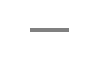
\begin{tikzpicture}  \draw[gray, ultra thick] (0,0) -- (0.5,0.0); \end{tikzpicture}). El perfil de densidad del agua está por fuera de la membrana (\textcolor{babyblueeyes}{azul} \begin{tikzpicture}  \draw[babyblueeyes, ultra thick] (0,0) -- (0.5,0); \end{tikzpicture}). En la interfase se localiza la densidad de grupos fosfato (\textcolor{orange}{naranja} 
\begin{tikzpicture}  \draw[orange, ultra thick] (0,0) -- (0.5,0); \end{tikzpicture}) y glicerol éster (\textcolor{darkgreen}{verde} \begin{tikzpicture}  \draw[darkgreen, ultra thick] (0,0) -- (0.5,0); \end{tikzpicture}). 

%%%%%%%%%%% Figura %%%%%%%%%%%%
\begin{figure}[t!]
%\vspace{0.5cm}
    \centering
	\includegraphics[width=0.8\linewidth, height=\textheight, keepaspectratio]{fig/02_dm/density_all.png} 
	\caption[Perfil de densidad de carga en las membranas lipídicas.]{Perfil de densidad de carga en las membranas lipídicas en función de la distancia \textit{z}. Las líneas más delgadas del sistema PCPG corresponden a las densidades de carga del POPG.}
      \index{density}
    \label{fig:densidad}
\end{figure}
%%%%%%%%%%%%%%%%%%%%%%% Fin %%%%%%%%%%%%%%%%%%%%%%%%

%%paper eze Chemistry and Physics of Lipids 213 (2018) 111–117
Una propiedad que se relaciona con la fluidez de la membrana es el \ac{apl}, a su vez esta propiedad está relacionada con el parámetro de orden de las colas hidrofóbicas del lípido, la compresibilidad y el empaquetamiento molecular \citep{Gapsys2013, Saeedimasine2019}. Además, el \ac{apl} también se puede emplear como un criterio para determinar si un sistema ha alcanzado el estado de equilibrio. La evolución del \ac{apl} en el tiempo se muestra en la \textbf{figura} \ref{fig:apl_zThick} (panel superior). Todos los sistemas alcanzan un estado de equilibrio desde los $\Xapprox$ 0.1 $\mu$s de simulación. \ac{dppc} presentó menor área promedio por lípido (68.8 \textpm 0.5 Å\textsuperscript{2}), valor que concuerda con lo reportado en literatura \citep{Petrache2000}. El sistema con mayor valor de \ac{apl} fue \ac{popg} con un promedio de 74.5 \textpm 0.5 Å\textsuperscript{2}, valor que concuerda con lo reportado en literatura \citep{Baoukina2012, Drabik2020, Kucerka2011, Shahane2019}. Respecto \ac{dppc}, es un lípido con un grupo polar más pequeño comparado al \ac{popg} que tiene un grupo polar con carga negativa, con un grupo polar más voluminoso y por tanto ocupa mayor área por molécula. En cuanto a los otros dos sistemas (\ac{popc} y PCPG), el \ac{apl} de PCPG es ligeramente mayor que \ac{popc} puro. 


La \textbf{figura} \ref{fig:apl_zThick} (panel inferior) muestra el espesor de la membrana (D$_{HH}$) para todos los sistemas simulados, este se determinó midiendo la distancia en \textit{z} entre los grupos fosfatos de la hemicapa superior e inferior \citep{Smith2021}. Los valores de D$_{HH}$  fueron similares con una mínima diferencia para \ac{dppc}. Además con este parámetro y el \ac{apl} se calculó el volumen por lípido, V$_{L} = \frac{APL\;x\;D_{HH}}{2}$. El orden del V$_{L}$ de mayor a menor fue: \ac{popg}>PCPG>\ac{popc}>\ac{dppc}. El V$_{L}$ es importante porque puede ser un indicativo para tener una idea del número de lípido que tienden a permanecer cerca del heterodímero $\alpha$IIb$\beta$3. Por lo tanto, es de esperarse que en el sistema  \ac{dppc} haya un mayor número de lípidos formando un anillo alrededor de los péptidos, mientras que para \ac{popg} deberían haber menos lípidos.
%%%%%%%%%%% Figura %%%%%%%%%%%%
\begin{figure}[t!]
    \centering
	\includegraphics[width=0.99\linewidth, height=\textheight, keepaspectratio]{fig/02_dm/ApL_zthickness_all.png} 
\caption[Área por lípido y espesor de membrana.]{Área por lípido y espesor de membrana.}
        \index{areaL}
    \label{fig:apl_zThick}
\end{figure}
%%%%%%%%%%%%%%%%%%%%%%% Fin %%%%%%%%%%%%%%%%%%%%%%%%

El parámetro de orden en modelo \ac{cg} (S$_{cc}$) para cada lípido se calculó con el programa \textit{LiPyphilic} \citep{Smith2021} empleando la ecuación \ref{ecu:scc},

\begin{equation}
S_{cc} = \frac{\langle 3 \cos^2 \theta \text{--}1 \rangle }{2}
\label{ecu:scc}
\end{equation}

donde el ángulo $\theta$ es el vector entre la normal a la membrana y el vector que conecta dos partículas \ac{cg} consecutivas. Los valores de \textit{S}$_{cc}$ para cada cadena hidrocarbonada se muestran en la \textbf{figura} \ref{fig:scc}. Los enlaces que están más próximos al grupo polar de los lípidos presentan mayor orden comparado a los enlaces de partículas en los extremos de la cadena hidrocarbonada. Además, se ve que todos los lípidos presentan un \textit{S}$_{cc}$ muy similar, excepto, la cadena ``sn1'' de \ac{dppc} que presenta valores ligeramente mayores indicando que la bicapa \ac{dppc} sería la membrana más compacta. Estos resultados concuerdan con lo observado anteriormente para \ac{apl} y V$_{L}$. La \textbf{tabla} \ref{tab:parame_lipid} resume estos párametros calculados.

%%%%%%%%%%% Figura %%%%%%%%%%%%
\begin{figure}[H]
    \centering
	\includegraphics[width=0.9\linewidth, height=0.9\textheight, keepaspectratio]{fig/02_dm/scc_all.png} 
\caption[Parámetro de orden de los lípidos]{Parámetro de orden de los lípidos. A) y B) hacen referencia a las cadenas hidrocarbonadas de cada lípido. Notar que C2A y C2B se resaltan en color diferente porque según el lípido de interés puede ser D2A y/o D2B. PCPG corresponde a la mezcla POPC:POPC 70\%:30\%.}
        \index{areaL}
    \label{fig:scc}
\end{figure}
%%%%%%%%%%%%%%%%%%%%%%% Fin %%%%%%%%%%%%%%%%%%%%%%%%

La \ac{rdf} se usó para identificar poblaciones de lípidos que se encuentran a una distancia menor a 20 \AA \,del heterodímero $\alpha$IIb$\beta$3 en plano \textit{xy}. La \textbf{figura} \ref{fig:rdf} muestra el perfil de las \ac{rdf}s de cada bicapa diferenciando entre hemicapa superior e inferior. Las distribuciones radiales de los lípidos en la hemicapa superior (\textbf{figura} \ref{fig:rdf}A) son ligeramente menores a las de la hemicapa inferior (\textbf{figura} \ref{fig:rdf}B) en el rango de 8 a 20 \AA \,. Esta diferencia incrementa a medida que los lípidos se encuentran lejos del heterodímero. En el rango de los 4 a 8 \AA \,,la bicapa de POPC presenta mayor densidad de lípidos cerca del heterodímero en la hemicapa inferior. Respecto a las otra bicapas, la distribución de lípidos es similar, aunque la RDF para los lípidos de POPG es ligeramente menor en ambas hemicapas. Los promedios de los parámetros de membrana anteriormente calculados se muestran en la \textbf{tabla} \ref{tab:parame_lipid}.

%%%https://gist.github.com/orbeckst/b611626e7640f399580e233195c6429c   cómo se calcula el RDF en MDAnalisys

%%%%%%%%%%% Figura %%%%%%%%%%%%
\begin{figure}[t!]
    \centering
	\includegraphics[width=0.8\linewidth, height=0.99\textheight, keepaspectratio]{fig/02_dm/rdfAll.png} 
	\caption[Función de distribución radial \textit{g(r)} para los lípidos respecto al heterodímero $\alpha$IIb$\beta$3.]{Función de distribución radial \textit{g(r)} para los lípidos respecto al centro de masa del segmento transmembrana del heterodímero $\alpha$IIb$\beta$3. A) y  B) corresponden a la hemicapa superior e inferior de la bicapa, respectivamente. La \textbf{figura} \ref{fig:rdf_allConverg} muestra el rango completo en la ordena \textit{x} de \textit{g(r)}.}
      \index{rdf}
    \label{fig:rdf}
\end{figure}
%%%%%%%%%%%%%%%%%%%%%%% Fin %%%%%%%%%%%%%%%%%%%%%%%%


%%%%%Tabla resumen membranas%%%%
\begin{table}[H]
  \begin{center}
%  \centering
  \caption[Resumen de los parámetros de membrana]{Resumen de los parámetros de membrana. Área molecular por lípido (APL), parámetro de orden  (S\textbf{\LARGE{$_{cc}$}}), espesor de membrana (D$_{HH}$) y volumen por lípido (V$_{L}$). El \ac{apl} y el D$_{HH}$ tienen un margen de error de \textpm 0.5 \AA\textsuperscript{2} y el S\textbf{\LARGE{$_{cc}$}} de \textpm 0.01.}
    \label{tab:parame_lipid}
  \begin{threeparttable}
 
    \begin{tabular}{l| c c c c}
      \toprule % <-- Toprule here
		Parámetro 					&  POPC	& POPG 	& PCPG 	& DPPC \\ 
      \midrule % <-- Midrule here
		APL (\AA\textsuperscript{2}) & 72.2 	& 74.5 	& 72.8 	& 68.8 \\ 

		S\textbf{\LARGE{$_{cc}$}} 					& 0.52 	& 0.53 	& 0.54	& 0.56 \\ 

		D$_{HH}$ (\AA) 					& 35.4 	& 35.6 	& 35.6 	& 36.3 \\
		V$_{L}$ (\AA\textsuperscript{3}) &1277.9 & 1326.1 & 1295.8 	& 1248.7  \\  
      \bottomrule % <-- Bottomrule here
    \end{tabular}
    \end{threeparttable}
  \end{center}
\end{table}
%%%%Fin tabla#%%%%%%%%%
\vspace{-0.5cm}

\section{Interacción lípido-péptido}

\begin{figure}[b!]
\vspace{0.5cm}
    \centering
	\includegraphics[width=0.99\linewidth, height=0.99\textheight, keepaspectratio]{fig/02_dm/lipid_pept_contac_all.png} 
	\caption[Contactos lípido-péptido durante la dinámica]{Contactos lípido-péptido durante la dinámica. A-B) Frecuencia de contactos lípido-péptido de $\alpha$IIb y $\beta$3 respectivamente. C) Secuencia del segmento TM del heterodímero $\alpha$IIb$\beta$3. Cada residuo en el eje \textit{x} incluye las frecuencias de las cuatro composiciones lipídicas estudiadas.}
      \index{lipid_resid_contact}
    \label{fig:lipid_pept_contac_all}
\end{figure}
%%%%%%%%%%%%%%%%%%%%%%% Fin %%%%%%%%%%%%%%%%%%%%%%%%

Con la función de distribución radial se identificaron poblaciones de lípidos alrededor del heterodímero $\alpha$IIb$\beta$3. Resulta importante identificar con qué residuos interaccionan los lípidos más cercanos. Se consideró como contacto a todas aquellas partículas (tipo BB) del heterodímero que estuvieran a una distancia $\leq$ 6.0 \AA \,de la partícula fosfato (PO4) de cada lípido, distancia usada ampliamente para considerar que existe un contacto \citep{Hedger2019, Corradi2018, Sica2021, Zhekova2023}.
La \textbf{figura} \ref{fig:lipid_pept_contac_all}A-B muestra la frecuencia normalizada de lípidos que permanecen a una distancia $\leq$ 6.0 \AA \,del heterodímero $\alpha$IIb$\beta$3 durantente toda la dinámica. Los residuos subrayados (\rule{0.5cm}{0.4pt}) en la \textbf{figura} \ref{fig:lipid_pept_contac_all}C  corresponden al segmento \ac{tm}, se resaltan algunos residuos en colores diferentes importantes para el análsis de contactos. Se observa mayor frecuencia de contactos lípido-$\alpha$IIb (\textbf{figura} \ref{fig:lipid_pept_contac_all}A) comparado con lípido-$\beta$3. Los residuos P$^{965}$, W$^{967}$, K$^{989}$,  F$^{992}$ y F$^{993}$ de $\alpha$IIb presentaron una ligera mayor frecuencia de contactos tuvieron con lípidos, particularmente preferencia por lípidos \ac{popc} (\begin{tikzpicture}
\filldraw[popc] (0,0) rectangle (0.5,0.2); 
\end{tikzpicture}).


Por otro lado, el péptido $\beta$3 interacciona con lípidos a través de los residuos I$^{693}$, V$^{695}$, K$^{716}$, T$^{720}$, y H$^{722}$. Sin embargo, la interacción se da principalmente con los lípidos \ac{popc} y la mezcla PCPG (\begin{tikzpicture} \filldraw[pcpg] (0,0) rectangle (0.5,0.2); 
\end{tikzpicture}), siendo casi nula la interacción con \ac{popg} (\begin{tikzpicture} \filldraw[popg] (0,0) rectangle (0.5,0.2); 
\end{tikzpicture}) y \ac{dppc} (\begin{tikzpicture} \filldraw[dppc] (0,0) rectangle (0.5,0.2); 
\end{tikzpicture}). Esto sugiere que la función de distribución radial descrita anteriormente para \ac{popg}  y \ac{dppc}  se localiza alrededor del péptido $\alpha$IIb. La \textbf{tabla} \ref{tab:lipid_pept_contac} resume el número de lípidos en contacto con cada péptido.

%%%%%Tabla lipid-contacts%%%%
\begin{table}[H]
\begin{center}
\centering
    \caption[Número de lípidos en contacto con los péptidos.]{Número de lípidos en contacto con los péptidos.}
    \label{tab:lipid_pept_contac}
    
  \begin{threeparttable}
	\begin{tabular}{@{}ccccc@{}}
\toprule
                                   & \textbf{POPC} & \textbf{POPG}   & \textbf{PCPG}   & \textbf{DPPC}  \\ \cmidrule(l){2-5} 
\multirow{-2}{*}{Péptido} &
  $\overline{x}$\textpm std &
  $\overline{x}$\textpm std &
  $\overline{x}$\textpm std &
  $\overline{x}$\textpm std \\ \midrule
{\color[HTML]{FE0000} $\alpha$IIb} & 19.8\textpm4.8 & 12.1\textpm4.5 & 16.9\textpm5.4 & 13.8\textpm5.3 \\ 
{\color[HTML]{3531FF} $\beta$3}    & 11.1\textpm3.9 & 1.4\textpm4.0  & 13.9\textpm5.4 & 0.9\textpm2.5  \\ \bottomrule
\end{tabular}
\end{threeparttable}
\end{center}
\end{table}
%%%%%FIN Tabla lipid-contacts%%%%
%\vspace{-0.5cm}

En la región interfacial \ac{tm}-\ac{ic} (\textbf{figura} \ref{fig:lipid_pept_contac_all}C) ambos péptidos presentan residuos cargados positivamente. La presencia de las lisinas K$^{989}$, K$^{994}$ en $\alpha$IIb y K$^{716}$ en $\beta$3 interaccionan con el grupo fosfato de los lípidos. Kim et al. identificaron que la interacción PO$_{4}^{\text{--}}$--K$^{716}$ interviene en el control del ángulo de cruce e inclinación del heterodímero TM-IC $\alpha$IIb$\beta$3 \citep{Kim2012}. Los autores también demostraron que una mutación de este residuo y otros, disrumpe el estado inactivo de la integrina. Contrario a esta posición, Zhu et al. sugieren que la mutación de la K$^{716}$ conduce a la activación de la integrina porque se disrumpen los puentes de hidrógeno entre la cadena lateral de la lisina y la cadena carbonada de $\alpha$IIb \citep{Zhu2009}. Los estudios por \ac{rmn} en micelas sugieren que los residuos K$^{716}$LLITIHD$^{723}$ en $\beta$3 y K$^{989}$VGFFKR$^{995}$ en $\alpha$IIb presentan interacciones péptido-péptido y  algunos residuos interaccionan con lípidos contribuyendo a la estabilidad del heterodímero. %%%integrinas_tesis%%% Además 
Además, $\alpha$IIb presenta el motivo G$^{991}$FFKR$^{995}$ altamente conservado en hélices $\alpha$ \ac{tm} y crucial en la dimerización \citep{Leung-Hagesteijn1994, OToole1994, Hughes1996}. %%2018_TESIS-Linking
En este motivo se observaron interacciones lípido-péptido en las cuatro membrana simuladas.
%Respecto a la región interfacial \ac{ec}-\ac{tm}, en estudios previos \citep{Lau2009, Yang2009} se reportó que el anillo aromático de los triptófanos W$^{967}$ y W$^{968}$


%%%paper de Samson 2021_ansell_occupancy
A partir de estos contactos lípido-péptido, podemos plantearnos qué tiempo permanecen en contacto estos lípidos con el péptido. La ocupancia de interacción es definida como la fracción de tiempo en la simulación donde la partícula fosfato permanece en contacto con una partícula de un residuo del heterodímero \citep{Ansell2021}. La \textbf{figura} \ref{fig:occupancy} muestra que \ac{popc} permanece más tiempo interaccionando con $\alpha$IIb comparado con $\beta$3. La ocupancia de la mezcla PCPG fue similar para los dos péptidos. Por último, \ac{popg} y \ac{dppc} interaccionan poco tiempo con ambos péptidos. Todos los valores fueron normalizados por el número total de lípidos.


%%%Figura en commun_result/lipid_protein_contact
%%%%%%%%%%% Figura %%%%%%%%%%%%
\begin{figure}[H]
    \centering
	\includegraphics[width=0.75\linewidth, height=0.3\textheight, keepaspectratio]{fig/02_dm/occupancy_all.png} 
	\caption[Ocupancia de los lípidos en contacto con cada péptido.]{Ocupancia de los lípidos en contacto con cada péptido.}
      \index{occupancy}
    \label{fig:occupancy}
\end{figure}
%%%%%%%%%%%%%%%%%%%%%%% Fin %%%%%%%%%%%%%%%%%%%%%%%%

\section{Orientación del heterodímero TM-IC $\alpha$IIb$\beta$3 en la bicapa lipídica}

La integrina $\alpha$IIb$\beta$3 en su estado inactivo se caracteriza por presentar una asociación con una configuración definida entre los segmentos TM. Datos obtenidos en bicelas por \ac{rmn} \citep{Lau2009} sugieren que en el heterodímero, los dos segmentos TM forman un ángulo de cruce de $\Xapprox$ 25\textdegree. En solución CD$_{3}$CN/H$_{2}$O este ángulo es de $\Xapprox$ 30\textdegree \,\citep{Yang2009}.\\
Para la asociación de hélices \ac{tm} se deben favorecer ciertas interacciones: \ac{vdw}, puentes de hidrógeno, iónicas, polares, lípido-lípido, lípido-proteína \citep{Fleming2001, Moore2008}. Algunos estudios sugieren que hay ciertos motivos (grupo de residuos) que son relevantes en el proceso de asociación hélice-hélice. Motivos que incluyen Pro, Asn, Asp, His, Gly, y SxxG, QxxS, se encuentran en algunas estructuras de proteínas  \ac{tm} que asocian hélices $\alpha$. Las 18 subunidades $\alpha$ de integrinas se caracterizan por presentar un motivo  \underline{X}xxxG, donde \underline{X} puede ser: S, A, G en su segmento \ac{tm}.
En este caso particular nos centramos en la $\alpha$IIb que presenta el motivo GxxxG \citep{Litvinov2019}, el cual desempeña una función importante en el proceso de asociación del heterodímero $\alpha$IIb$\beta$3, además de contribuir en el ángulo de cruce entre las dos hélices. Por lo tanto, es importante estudiar cuál es la función del ambiente lipídico en la asociación del heterodímero y la orientación de cada uno de los segmentos en la membrana. A modo de ilustración, la \textbf{figura} \ref{fig:tilt_angle_all}A muestra el ángulo $\tau$ que se forma entre la normal de la membrana y eje principal de la hélice $\alpha$. La  \textbf{figura} \ref{fig:tilt_angle_all}B ilustra el ángulo de cruce entre dos hélices \ac{tm}. En la \textbf{figura} \ref{fig:tilt_angle_all}C se muestra algunas capturas a diferentes tiempos donde se observa visualmente la variación de los ángulos. La \textbf{figura} \ref{fig:lipid_pept_contac_all}C resalta el motivo GxxxG en $\alpha$IIb que proporciona estabilidad al heterodímero. Experimentalmente, se ha demostrado que la G$^{972}$ interacciona con V$^{700}$ y M$^{701}$ en $\beta$3, la G$^{976}$ con I$^{704}$. Además, la G$^{708}$ interacciona con las L$^{979}$ y L$^{980}$ de $\alpha$IIb que contribuyen en el cierre del ángulo de cruce del heterodímero \citep{Lau2009, Yang2009}.

%%%Figura en tesis_main/03_Figures/tilt/popc
%%%%%%%%%%% Figura %%%%%%%%%%%%
\begin{figure}[H]
    \centering
	\includegraphics[width=0.9\linewidth, height=0.6\textheight, keepaspectratio]{fig/02_dm/tilt_angle_all.pdf} 
	\caption[Esquema inclinación del heterodímero $\alpha$IIb$\beta$3 respecto a la normal de la bicapa.]{Esquema inclinación del heterodímero $\alpha$IIb$\beta$3 respecto a la normal de la bicapa.}
      \index{tilt_angle_all}
    \label{fig:tilt_angle_all}
\end{figure}
%%%%%%%%%%%%%%%%%%%%%%% Fin %%%%%%%%%%%%%%%%%%%%%%%%

El ángulo promedio de cruce entre las dos hélices \ac{tm} fue $\Xapprox$ 33.5\textdegree \,en las cuatro membranas. Este resultado concuerda con los reportados experimentalmente \citep{Lau2009, Yang2009}. También por simulaciones \ac{dm} han reportado un valor promedio de 30\textdegree \,simulado en una bicapa de \ac{dppc} \citep{Kalli2011}. Experimentalmente no se ha determinado con precisión un valor del ángulo de inclinación, sin embargo, los valores estimados varían de 20\textdegree \, a 30\textdegree \, para $\beta$3 y 0\textdegree \, a 10\textdegree \,para $\alpha$IIb \citep{Lau2008, Lau2008a}. Por simulaciones se informaron valores de de 5\textdegree \, y 30\textdegree \,para $\alpha$IIb y $\beta$3, respectivamente \citep{Kalli2011}. En otro estudio Antreas Kalli obtuvo valores de $\alpha$IIb $\Xapprox$ 15\textdegree \,y $\beta$3 $\Xapprox$ 27\textdegree \,\citep{Kalli2013} por simulaciones de DM. El ángulo de inclinación de cada péptido es diferentes en las cuatro membranas lipídicas (\textbf{figura} \ref{fig:angles}).

%%%%%%%%%%% Figura %%%%%%%%%%%%
\begin{figure}[H]
    \centering
	\includegraphics[width=1\linewidth, height=0.99\textheight, keepaspectratio]{fig/02_dm/angles.png} 
	\caption[Distribución del ángulo de cruce del heterodímero $\alpha$IIb$\beta$3 y ángulos de inclinación de cada péptido respecto a la normal de la bicapa]{Distribución del ángulo de cruce del heterodímero $\alpha$IIb$\beta$3 y ángulos de inclinación de cada péptido respecto a la normal de la bicapa. Rojo y azul se corresponden a la distribución de ángulo de inclinación de $\alpha$IIb y $\beta$3, respectivamente. En verde la distribución del ángulo de cruce entre las hélices \ac{tm}.}
      \index{angles}
    \label{fig:angles}
\end{figure}
%%%%%%%%%%%%%%%%%%%%%%% Fin %%%%%%%%%%%%%%%%%%%%%%%%

%%%2018-TESIS
Un análisis más detallado de cada sistema se resume en los mapas de contactos entre los dos péptidos durante la dinámica, ver \textbf{figura} \ref{fig:contact_map}. El eje \textit{y} de cada mapa corresponde a los residuos del péptido $\alpha$IIb y el eje \textit{x} a $\beta$3. La escala a blanco (poca o nula interacción) y negro (alta interacción) representa los contactos entre determinados residuos. Al medio de los mapas de contacto se muestra parte de la estructura secundaria del $\alpha$IIb$\beta$3 y algunos residuos destacados para durante el análisis, esta representación corresponde a la secuencia que se muestra en la \textbf{figura} \ref{fig:contact_map}E. La diferencia más notable entre los cuatro sistemas se observa con \ac{dppc} (\textbf{figura} \ref{fig:contact_map}D). Varios contactos interaccionan menos tiempo en comparación a las otras membranas y también se observan contactos nuevos respecto a los otros sistemas. Por ejemplo, en la región interfacial EC-TM contactos como W$^{968}$--V$^{696}$, W$^{968}$--V$^{700}$, V$^{969}$--L$^{697}$, V$^{969}$--V$^{700}$ y V$^{969}$--A$^{703}$ interaccionan menos tiempo en DPPC. En esta misma región hay contactos de baja frecuencia (gris claro) que no vemos en los demás ambientes lipídicos: P$^{965}$--V$^{696}$, P$^{965}$--L$^{697}$, P$^{965}$--V$^{700}$, I$^{966}$--L$^{694}$ y I$^{966}$--L$^{697}$. Continuando en la diagonal del mapa de contactos del mismo sistema DPPC, el motivo GxxxG en $\alpha$IIb presenta contactos de baja frecuencia con residuos de $\beta$3 (\begin{tikzpicture}  \draw[deeppink, ultra thick, dotted] (0,0) -- (0.8,0.0); \end{tikzpicture}). En todos los sitemas se consevaron los contactos entre G$^{976}$--I$^{704}$ y L$^{980}$--G$^{708}$, mientras que los contactos que forma la G$^{972}$, G$^{976}$, L$^{979}$ con otros residuos de $\beta$3 disminuyeron en tiempo de interacción respecto a los otros sistemas. Además, hay nuevos contactos de baja frecuencia, por ejemplo: V$^{973}$--V$^{700}$, L$^{975}$--I$^{704}$, G$^{977}$--G$^{708}$, L$^{980}$--L$^{705}$. Se han realizado mutaciones del motivo GxxxG en $\alpha$IIb y de la G$^{708}$ en $\beta$3 \citep{Li2005, Luo2005}, concluyendo que cualquier mutación sobre este motivo disrumpe el ensamble de las hélices induciendo la activación de la integrina. Continuando hacia abajo en la diagonal, otros contactos con menor fecuencia de interacción durante la dinámica son: V$^{984}$--L$^{712}$, L$^{985}$--W$^{715}$ y M$^{987}$--L$^{712}$; éstos tres contactos son bien conservados en las otras tres bicapas. Más cerca a la región interfacial TM-IC los contactos M$^{987}$--I$^{719}$  (\begin{tikzpicture}  \draw[orange, ultra thick, dotted] (0,0) -- (0.8,0.0); \end{tikzpicture}) y G$^{991}$--I$^{719}$ son los únicos que se conservan en las bicapas excepto en DPPC que disminuye su frecuencia de interacción. Ésta región es la que mayor diferencia presenta en los cuatro sistemas. Observemos en DPPC (\textbf{figura} \ref{fig:contact_map}D, inferior derecha) el residuo I$^{719}$ en $\beta$3 además de interaccionar con M$^{987}$ y G$^{991}$, también interacciona con una frecuencia intermedia con F$^{993}$, similar a POPC sin embargo, este contacto es fuertemente marcado en las bicapas de POPG y PCPG.
Otro contacto ampliamente estudiado que es relevante en el proceso de activación de la intergina es el puente salino formado entre la R$^{995}$ en $\alpha$IIb y el D$^{723}$ en $\beta$3 (\begin{tikzpicture}  \draw[blue, ultra thick, dotted] (0,0) -- (0.8,0.0); \end{tikzpicture}) \citep{Yang2009, Lau2008a, Favier2018, Partridge2005}. En la membrana \ac{dppc}, ésta interacción presenta baja frecuencia respecto a los otros sistemas. Estas diferencias podrían explicar por qué las distribuciones de los ángulos de inclinación y cruce entre las hélices \ac{tm} (\textbf{figura} \ref{fig:tilt_angle_all}B) son dispersas y toman un rango de valores muy amplio en DPPC. 
En la mezcla lipídica PCPG (\textbf{figura} \ref{fig:contact_map}C) la presencia de un 30\% de \ac{popg} en la membrana de \ac{popc} fortalece el contacto del puente salino R$^{995}$--D$^{723}$ siendo así el ambiente lipídico en el que permanece más tiempo en interacción. Además, la H$^{722}$ de $\beta$3 fortaleció notablemente su interacción con K$^{994}$ y R$^{995}$ en $\alpha$IIb (\textbf{figura} \ref{fig:contact_map}C, recuadro pequeño en rojo). Por el contrario un contacto que se pierde por completo fue F$^{993}$--H$^{722}$ donde la frecuencia de interacción se da en el siguiente orden \ac{popg}>\ac{popc}>PCPG. Los contactos K$^{994}$--L$^{718}$ y K$^{994}$--I$^{719}$ son los que duran más tiempo interaccionando respecto a los demás sistemas. El contacto F$^{993}$--I$^{719}$ no se observa en la 

%%%%%%%Hoja horizontal %%%%%%%%%%%%%%%%%%%%%%%%
\begin{landscape}
%%%%%%%%%%% Figura %%%%%%%%%%%% 
\begin{figure}[b]
 \centering
	\includegraphics[width=1\linewidth, height=1.2\textheight, keepaspectratio]{fig/02_dm/contact_map.png}
	\caption[Mapa de contactos entre residuos del segmento \ac{tm}-\ac{ic} $\alpha$IIb y $\beta$3 en bicapas lipídicas]{Mapa de contactos entre residuos del segmento \ac{tm}-\ac{ic} $\alpha$IIb y $\beta$3 en bicapas lipídicas. E) Secuencia de residuos importantes en el análisis de contactos.}
        \index{contact_map}
    	\label{fig:contact_map}
\end{figure}
\end{landscape}
%%%%%%%%%%%%%%%%%%%%% Fin %%%%%%%%%%%%%%%%%%%%%%%

\noindent membrana POPG y presenta baja frecuencia en las membranas POPC y DPPC.
Las demás interacciones se conservan de forma similar a cuando los péptidos se encuentran en una bicapa pura de \ac{popc} o \ac{popg}.


Comparando los sistemas \ac{popc} y \ac{popg}, la mayoría de los contactos entre las hélices son similares, sin embargo, en la región próxima a la TM-IC algunos contactos son más estables en \ac{popg} respecto al \ac{popc}. La F$^{993}$ de subunidad $\alpha$IIb permanece más tiempo en contacto con la H$^{722}$ y la I$^{719}$ de $\beta$3 a su vez, la F$^{993}$ interacciona más tiempo con la L$^{718}$ en $\beta$3. El puente salino R$^{995}$ en $\alpha$IIb y el D$^{723}$ en $\beta$3, también permanece más tiempo en contacto en la membrana de \ac{popg}, además, estos residuos interaccionan más tiempo con otros residuos cuando se encuentran en la membrana con carga negativa. La R$^{995}$ interacciona con I$^{719}$ y T$^{720}$; el D$^{723}$ de $\beta$3, interacciona por un tiempo más prolongado con F$^{998}$ y F$^{999}$. Por último, en \ac{popg} los residuos K$^{725}$, E$^{726}$ y F$^{727}$ de $\beta$3 interaccionan con la secuencia N$^{996}$--RPPL--$^{1000}$. Este pequeño cúmulo o clúster de interacciones se observa levemente en los otros tres sistemas simulados. Observando la estructura secundaria de cada péptido (\textbf{figura} \ref{fig:tm_domain}A-B), la subunidad $\alpha$IIb no tiene estructura definida en el segmento \ac{ic}, por lo tanto, esta región presenta alta flexibilidad, confiriendo mayor grado de libertad a los residuos para explorar diferentes posiciones espaciales. 

La \textbf{figura} \ref{fig:distance_contacts_all} muestra la distribución de las distancias de enlace de algunas de las interacciones mencionadas anteriormente. La distancia de enlace R$^{995}$--D$^{723}$, en la bicapa de \ac{dppc} es donde presenta mayor heterogeneidad con tendencia a tomar valores mayores a 6.0 \AA. Por el contrario, las distancias más cortas se observan en la bicapa PCPG, ésto concuerda con lo observado en el mapa de contactos (\textbf{figura} \ref{fig:contact_map}C) en donde se muestra una prolongada interacción. Las distribuciones de las interacciones G$^{972}$--V$^{700}$ y G$^{972}$--A$^{700}$ y G$^{972}$--I$^{704}$ son relativamente similares en todas las membranas, excepto en DPPC que su distribución esta ligeramente sesgada a valores > \, 6.5 \AA.  

%%%%%%%%%%% Figura %%%%%%%%%%%%
\begin{figure}[H]
\vspace{0.5cm}
    \centering
	\includegraphics[width=0.9\linewidth, height=0.99\textheight, keepaspectratio]{fig/02_dm/distance_contacts_all.png} 
	\caption[Distribución de las distancias de enlace de algunas interacciones entre residuos del heterodímero \ac{tm}-\ac{ic} $\alpha$IIb$\beta$3.]{Distribución de las distancia de enlace de algunas interacciones entre residuos del heterodímero \ac{tm}-\ac{ic} $\alpha$IIb$\beta$3.}
      \index{distance_contacts_all}
    \label{fig:distance_contacts_all}
\end{figure}
%%%%%%%%%%%%%%%%%%%%%%% Fin %%%%%%%%%%%%%%%%%%%%%%%%


\section{Discusión del capítulo}

%%%%2017_Helix-helix
	Se han realizado varios estudios enfocados en la interacción hélice-hélice de la integrinas. Algunas de las técnicas experimentales empleadas son FRET y RMN en micelas de detergentes, bicelas y liposomas \citep{Mineev2014, Merzlyakov2006}. Estos estudios se enfocan principalmente en el efecto de la sustitución de residuos en la asociación de las hélices TM. Se encontró que en muchos casos las mutaciones causan la activación de la integrina, esto significa que disminuye la propensión a la formación del heterodímero de hélices $\alpha$ TM, aunque también se han observado mutaciones que inducen en estado inactivo de la integrina \citep{Lau2009}. Sin embargo, el efecto del ambiente lipídico no ha sido considerado en este proceso biológico. Por otra parte, varios estudios sugieren que las propiedades de los lípidos en la bicapa son importantes en la termodinámica de asociación y dimerización de proteínas de membrana. Por ejemplo, se ha observado que la fase gel de la membrana tiene un impacto favorable en la energía libre de la interacción hélice-hélice comparado a membranas con la fase líquido cristalino \citep{Anbazhagan2010}. Una razón por la cual se debe esta mejora de la dimerización en la fase gel más ordenada es el mayor costo energético de la incorporación de una hélice de proteína en ella, esto que hace que el estado dimérico con una superficie más pequeña sea más preferible.

	Hemos mencionado que el segmento \ac{tm} de $\alpha$IIb$\beta$3 es relevante para el proceso de activación de la integrina. En este capítulo se obtuvo información relevante acerca de cómo el ambiente lipídico regula la orientación del segmento \ac{tm} de $\alpha$IIb$\beta$3. Respecto a la \textbf{interacción lípido-péptido} el orden de interacción y ocupancia (porcentaje de tiempo que permanece en contacto) lípido-$\alpha$IIb fue POPC>PCPG>POPG>DPPC, mientras que lípido-$\beta$3 fue POPC>PCPG\(>\!\!>\)POPG>DPPC. En los dos péptidos la interacción con los lípidos se favorece más en la región interfacial TM-IC (hemicapa superior) comparado a la región interfacial TM-EC (hemicapa inferior). Esta diferencia de número de contactos lípido-péptido entre las hemicapas está influenciada por la flexibilidad de los segmentos IC de cada péptido que le permite a los residuos de la interfaz explorar diferentes posiciones en el espacio.	
	El grupo polar de los lípidos también influye en la asociación de hélices TM: lípidos aniónicos forman dímeros menos estables \citep{Hong2011}. Estas interacciones pueden verse de forma dualista: ya sea como la dimerización de la integrina $\alpha$IIb$\beta$3 que hace que la proteína adapte el entorno lipídico a sus preferencias, o como ciertos entornos lipídicos que favorecen la asociación de $\alpha$IIb$\beta$3. En rigor, estos puntos de vista son complementarios entre sí y ambos efectos se producen al mismo tiempo. La \textbf{figura} \ref{fig:rdf}B muestra la preferencia de lípido POPC y DPPC a localizarse más cerca al heterodímero comparado a la membrana de POPG.
		
	 Algunos de los residuos de $\alpha$IIb que interaccionan con lípidos son: W$^{967}$, K$^{989}$, V$^{990}$, F$^{992}$ y F$^{993}$; en $\beta$3 los contactos más relevantes fueron con los residuos: K$^{716}$, T$^{720}$ (ver \textbf{figura} \ref{fig:lipid_pept_contac_all}A-B). Éstos contactos lípido-péptido pueden influir en la conformación y orientación individual de cada péptido así como en la estabilidad segmento TM \citep{Stangl2015}. Además, el grupo de residuos K$^{989}$VGFFK$^{994}$ interacciona con lípidos y se ha reportado que contribuye en ángulo de cruce entre los dos segmentos TM \citep{Lau2008,Zhu2009}, por lo tanto, acá se podría alterar la estabilidad del heterodímero. Además, interacciones no específicas de lípidos también son comunes en las membranas biológicas. Por ejemplo, lípidos con cadenas de carbono insaturadas tienden a localizarse cerca de las hélices TM \citep{Flinner2015}. Esto va en el mismo sentido a lo observado con lípidos de POPC y DPPC cerca de los heterodímeros. POPC se ordena alrededor péptidos TM a través de la formación de una capa lipídica ordenada más grande, que es en muchos aspectos análogo al efecto hidrofóbico de las proteínas de membrana solubles en un ambiente acuoso \citep{Bocharov2017}. Interacciones electrostáticas se han estudiado entre la R$^{995}$ y lípidos como POPS y PIP2 \citep{Orowski2015, Schmidt2015}. En ambos estudios la interacción R$^{995}$-lípido disrumpen el puente salino entre R$^{995}$ en $\alpha$IIb y D$^{723}$ en $\beta$3.

	Las hélices TM tienen una orientación preferente relativa al plano de la membrana. Para cada péptido se calculó el de inclinación respecto a la normal de la membrana y el ángulo de cruce entre las dos hélices TM.  El motivo G$^{972}$xxxG$^{976}$ en $\alpha$IIb desempeña una función importante en la determinación de este ángulo entre las dos hélices TM y como mencionaremos más adelante, los contactos que forma este motivo con residuos de $\beta$3 no se vieron significativamente alterados, excepto en la membrana DPPC. Los ángulos de inclinación de cada péptido presentaron diferencias entre una membrana y otra, específicamente cuando se encuentra en un ambiente de DPPC. Incluso en DPPC el ángulo de cruce explora posiciones con ángulos de inclinación menores a 30\textdegree \,y mayores a 40\textdegree . Con base en estos resultados vemos cómo la inclinación de los péptidos es modifica según la composición de la membrana. 
Experimentalmente se ha reportado que el ángulo de inclinación de $\beta$3 se mantiene oscilando entre 25\textdegree \,y 30\textdegree \,. En esta orientación la cadena lateral con carga positiva de la K$^{716}$  interacciona con el grupo polar negativo del fosfato cerca de la interfaz membrana-agua \citep{Lagarrigue2016}. Un cambio en el ángulo de inclinación causada por la pérdida de la orientación de la K$^{716}$ puede disrumpir el heterodímero $\alpha$IIb$\beta$3 e inducir la activación de la integrina. 

	%%%2015_Orlowski
	Por lo general, el segmento TM de las integrinas presenta dos regiones de interacción que estabilizan la conformación inactiva del heterodímero. Una de ellas es la que se establece entre el motivo altamente conservado G$^{991}$FFKR$^{995}$ de $\alpha$IIb y los residuos hidrofóbicos W$^{715}$ e I$^{719}$ de $\beta$3, siendo estabilizada por el puente salino R$^{995}$--D$^{723}$. Estas interacciones se conocen como cierre de la membrana interna (CMI). En el extremo opuesto de la membrana (hemicapa superior), la interacción entre G$^{708}$ de $\beta$3 y el motivo G$^{972}$xxxG$^{976}$ en $\alpha$IIb se denomina cierre de la membrana externa (CME). Es crucial destacar que las mutaciones en los residuos de cualquiera de estos sitios de interacción (CMI y CME) resultan en interacciones perturbadas de las hélices TM, lo que puede llevar a una integrina constantemente activa \citep{Ye2014, Lau2009}.
	Del análisis del mapa de \textbf{contactos péptido-péptido} se obtuvo información relevante que permite comprender cómo se ven alterados y/o se forman contactos entre los segmentos TM del heterodímero $\alpha$IIb$\beta$3. La región CMI del heterodímero $\alpha$IIb$\beta$3 presentó la mayor alteración en contactos péptido-péptido en las cuatro composiciones lipídicas estudiadas. En particular resulta relevante la función del ambiente lipídico en la interacción tipo puente salino entre R$^{994}$ en $\alpha$IIb y  D$^{723}$ en $\beta$3. En la membrana que menos se favorece dicha interacción es DPPC y se fortalece en PCPG. En este sentido DPPC fue la membrana que más alteró contactos del péptido-péptido comparado a los otros tres sistemas. Los contactos que forma el motivo G$^{972}$xxxG$^{976}$ con algunos residuos de $\beta$3 se mantuvieron durante toda la simulación, excepto en la membrana DPPC que se vieron afectados, particularmente las interacciones G$^{972}$--V$^{700}$ y L$^{979}$--G$^{708}$, y esta diferencia respecto a los observado en las otras tres membranas va en el mismo sentido de lo observado con las diferencias en las distribuciones de los ángulos de inclinación de cada péptido. Por lo tanto, podemos decir que el DPPC altera notablemente interacciones péptido-péptido, sin embargo, éstas modificaciones no logran la separación del heterodímero. 